\pdfoutput=1
\documentclass[11pt]{article}
\usepackage{eurosym}
\usepackage[final]{acl}
\usepackage{times}
\usepackage{latexsym}
\usepackage[T1]{fontenc}
\usepackage{graphicx}
\usepackage[utf8]{inputenc}
\usepackage{microtype}
\usepackage{multirow}
\usepackage{subcaption}



\title{University of Bucharest Team at Semeval-2022 Task4: Detection and
	Classification of Patronizing and Condescending Language}

\author{Raluca Andreea G\^inga, {\bf Bogdan Dobre},  \\  {\bf Tudor-Andrei Dumitra\c{s}cu} \and {\bf Bogdan Radu Silviu Sielecki}\\
University of Bucharest \\
\texttt{\{gingaraluca, dobrebogdan98, }\\
\texttt{tudorandrei.dumitrascu, sieleckiradu\}@gmail.com }
}

\begin{document}
\maketitle

\begin{abstract}
	This paper details our implementations for finding Patronizing and
	Condescending Language in texts, as part of the SemEval Workshop Task 4.
	We have used a variety of methods from simple machine learning algorithms applied
	on bag of words, all the way to BERT models, in order to solve the binary classification
	and the multi-label multi-class classification.
\end{abstract}

\section{Introduction}

The Patronizing and Condescending Language Detection Task \cite{perezalmendros2022semeval} is based on the
paper Don't Patronize Me! \cite{perezalmendros2020dont}, which is an annotated Dataset with Patronizing and
Condescending Language Towards Vulnerable Communities.

The aim of this task is to identify PCL, and to categorize the language
used to express it, specifically when referring to communities
identified as being vulnerable to unfair treatment in the media.

Participants were provided with sentences in context (paragraphs), extracted
from news articles, in which one or several predefined vulnerable
communities are mentioned. The challenge is divided into two subtasks.

\begin{enumerate}
	\item Subtask 1: Binary classification. Given a paragraph, a system must
	      predict whether or not it contains any form of PCL.

	\item Subtask 2: Given a paragraph, a system must identify which PCL
	      categories express the condescension. The PCL taxonomy was defined
	      based on previous works on PCL (i.e. Unbalanced power relations, Shallow
	      solution, Presupposition, Authority voice, Metaphor, Compassion, The poorer,
	      the merrier. )
\end{enumerate}


\section{Background}

The dataset used for this SemEval 2022 task was Don't Patronize Me! \cite{perezalmendros2020dont},
which contains a suite of sentences that mention some vulnerable communities
and published in media in a lot of English speaking countries. The
paragraphs were manually annotated to show 1) whether the text contains any
kind of PCL, and 2) if it contains PCL, what linguistic techniques
(categories) are used to express the condescension. The paragraphs, according to \cite{perezalmendros2020dont}, were extracted from News on Web (NoW) corpus \cite{davies}, being annotated by three expert annotators, with backgrounds in communication, media and data science.

The dataset for subtask 1 (binary classification) contained a number of
10.636 paragraphs and 2.792 instances were used for the categories
classification subtask.

In Figure \ref{fig1}, it can be seen that for the first subtask, there are almost
1000 texts that contain PCL. This means that the dataset is highly imbalanced and this problem needs to be addressed.

% DONE: Remove the photos if we're not mentioning or discussing them

\begin{figure}[ht]
	\centering
	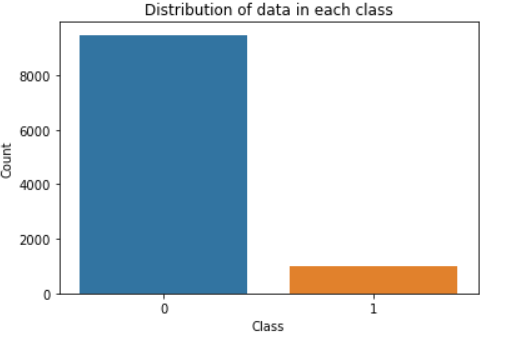
\includegraphics[width=0.4\textwidth]{DataDistribution.png}
	\caption{Classes Distribution for Binary Classification problem (Subtask 1)}
	\label{fig1}
\end{figure}


For task 2, the paragraphs from task 1 are split according to the type of PCL speech category into sentences, resulting in 950 samples.

\section{System Overview}

\begin{enumerate}

	\item Subtask 1 (Binary Classification)

	      Because the dataset was very imbalanced, we tried different approaches in
	      order to make it balanced:

	      \begin{itemize}
		      \item Adding a class weight to the models used. In this approach, we
		            computed a metric in which we obtained a class weight according to the
		            imbalance of the dataset. Through this method, we gave some different
		            weights to both the majority and minority classes. This whole process had
		            the purpose to penalize the miss classification made by the minority class by
		            setting a higher class weight and at the same time, reducing the weight for
		            the majority class.

		      \item Using oversampling methods and special ensemble techniques. In this
		            approach, we used methods like SMOTE (Synthetic Minority
		            Over-sampling Technique) \cite{Chawla_2002}, Adasyn (Adaptive Synthetic) \cite{4633969}, SVM-SMOTE \cite{7392251} and SPE (Self-Paced Ensemble) \cite{Liu_2020} that performs strictly balanced under-sampling in each
		            iteration, being very efficient computationally.

		      \item Augmenting the data. Because we notice so little data for label 1, we
		            decided to collect hate speech datasets from Kaggle\footnote{\href{https://www.kaggle.com/search?q=hate+speech+in\%3Adatasets}{Hate Speech datasets}} and add the positive texts into our
		            dataset in order to balance the classes frequency, obtaining a total of 6372
		            from 795 initial texts with label 1. We will notice in the results section
		            that this collection and generation of new dataset did not provide good
		            results.
	      \end{itemize}

	      The dataset was preprocessed. The preprocessing consisted in: clearing the special characters, lowercasing, tokenization, stopwords removal, removing the words shorter than 3 characters. Then, the resulted (and clean) dataset was split into two preprocessed
	      types: lemmatized cleaned dataset and stemmed cleaned dataset. These two
	      datasets were generated in order to make some comparison between those two
	      techniques and to see which provided the best results.

	      To extract features from text, we have used TF-IDF \cite{ref1}, Keras Tokenizer\footnote{\href{https://www.tensorflow.org/api_docs/python/tf/keras/preprocessing/text/Tokenizer}{Tokenizer method brought by Keras}}, Word2Vec with Skip-Gram \cite{mikolov2013word2vec} and, finally, Bert Tokenizer provided by Hugging Face \cite{huggingface}.

	      We have also used a variety of models such as Neural Networks with 3 dense layers, Long Short
	      Term Memory (LSTM) \cite{hichreichter} with 64 and 128 neurons with dropout of 0.1 as well, basic
	      Machine Learning algorithms like Logistic Regression, Random Forest, Support
	      Vector Machines as XGBoost. In the end, we decided to try BERT embeddings
	      and a BERT classification model, BertForSequenceClassification \footnote{\href{https://huggingface.co/docs/transformers/model_doc/bert\#transformers.BertForSequenceClassification}{Bert for Sequence Classification}}, that
	      contains a single linear classification layer on top and that provided the
	      best results after all of the other approaches.

	      Another approach, called "Text shards" made use of the subtask related to
	      multi-class classification as well. For an average text that contains PCL,
	      only some small pieces of them are actually PCL and the rest of the text are
	      not. The assumption is that this confuses the model, because a combination
	      of PCL and non-PCL is labeled as PCL. To address this, the following
	      approach is used:

	      \begin{itemize}
		      \item negative examples are left as they are

		      \item each positive example is replaced with the actual pieces of PCL inside
		            it that we can get from the categories file

		      \item the positive examples obtained this way are added with the negative
		            examples to obtain a training dataset

		      \item all the sentences are cleaned of characters that are not letters and
		            the words in each sentence are lemmatized

		      \item a Tensorflow Hub pretrained model called Universal Sentence Encoder \cite{USE} is
		            trained on it

		      \item for each text that we want to predict, we first use the model on the
		            whole text to get an initial label

		      \item a window (of the size of the average length of a cleaned PCL fragment
		            * 2) is slided through the text and the model is used to predict that
		            particular substring. If it is labeled as PCL, then we consider the whole
		            text as PCL.
	      \end{itemize}

	\item Subtask 2 (Multi-label Multi-class Classification)

	      Considering the fact that the vocabulary of the is English is large,
	      we have tried to leverage the power of pretrained language models.
	      Therefore we have chosen 3 BERT-based models which were pretrained
	      for hate speech detection and sentiment analysis. The BERT models
	      also provided a tokenizer which split the sentences into tokens and
	      appended the required tokens. The BERT models are used from the
	      transformers library \cite{huggingface}.

	      \begin{itemize}
		      \item BERT \cite{bert} Uncased

		      \item  BERT Multilingual Uncased

		      \item BERT HateXplain \cite{mathew2020hatexplain}: This model was
		            trained to classify text as Hate speech, Offensive or Normal.
		            It was trained on Gab, Twitter and Humain Rationale;

		      \item Distil BERT : This model is a version of Distilled BERT
		            finetuned on the Twitter dataset;

		      \item Distil BERT Multilingual Cased \cite{DistilBERT}

		      \item Distill RoBERTa : This model is a version of Distilled
		            RoBERTa finetuned on the Twitter dataset;
	      \end{itemize}

	      In the paper describing the dataset \cite{perezalmendros2020dont},
	      the authors group the categories into 3 General categories.

	      \begin{enumerate}
		      \item The saviour: Unbalanced power relations and Shallow relations

		      \item The Expert: Presupposition and Authority voice

		      \item The Poet: Compassion, Metaphor and The poorer the merrier

	      \end{enumerate}

	      From this idea, we tried to train the models to predict those 3
	      categories, and save the hidden features to a fixed latent space.
	      Then these learned features can be used when training the model to
	      predict the required 7 sub-classes.

	      Along with those BERT-based model, we also tried to implement models
	      based on Word2Vec \cite{mikolov2013word2vec} (trained on "Google News")
	      and Machine Learning algorithms based on TF-IDF and BOW:

	      \begin{itemize}
		      \item LSTM Word2Vec Embeddings \cite{staudemeyer2019understanding}
		      \item BiLSTM Word2Vec Embeddings \cite{huang2015bidirectional}
		      \item RNN Word2Vec Embeddings \cite{rnn}
		      \item SVM TF-IDF
		      \item RandomForest TF-IDF
	      \end{itemize}

	      We also dabbled with the thought of training our own Word2Vec, in
	      order to create a model specialized on hate speech. However we
	      decided against this idea, due to the lack of usable datasets and the
	      computational resources required for this task.


\end{enumerate}


\section{Results}


\begin{table*}\small
	\centering
	\begin{subtable}{1\textwidth}
		\centering
		\begin{tabular}{lcccc}
			\hline \textbf{Approach $\backslash$ Dataset} & Simple        & SPE  & SMOTE         & SVM-SMOTE     \\ \hline
			Neural Networks                               & 0.27          & -    & 0.2823        & 0.3187        \\
			Logistic Regression                           & \textbf{0.34} & -    & \textbf{0.35} & \textbf{0.35} \\
			Random Forest                                 & 0.067         & 0.31 & 0.19          & 0.16          \\
			Support Vector Machines                       & 0.27          & -    & 0.10          & 0.14          \\
			XGBoost                                       & 0.15          & -    & 0.23          & 0.24          \\
			\hline
		\end{tabular}
		\caption{Results on Imbalanced and Oversampled Lemmatized dataset}
	\end{subtable}
	\bigskip
	\begin{subtable}{1\textwidth}
		\centering
		\begin{tabular}{lcccc}
			\hline \textbf{Approach $\backslash$ Dataset} & Simple        & SPE  & SMOTE         & SVM-SMOTE     \\ \hline
			Neural Networks                               & 0.2698        & -    & 0.289         & 0.3166        \\
			Logistic Regression                           & \textbf{0.35} & -    & \textbf{0.38} & \textbf{0.37} \\
			Random Forest                                 & 0.038         & 0.31 & 0.21          & 0.13          \\
			Support Vector Machines                       & 0.27          & -    & 0.14          & 0.20          \\
			XGBoost                                       & 0.17          & -    & 0.23          & 0.24          \\
			\hline
		\end{tabular}
		\caption{Results on Imbalanced and Oversampled Stemmed dataset}
	\end{subtable}
	\caption{ Results on Imbalanced and Oversampled Lemmatized \& Stemmed dataset. The results are in terms of \textit{f1\_score}. }
	\label{table1}
\end{table*}

\begin{table}\small
	\centering
	\begin{tabular}{lrl}
		\hline \textbf{Approach $\backslash$ Dataset} & Augmented dataset \\ \hline
		Neural Networks                               & 0.2155            \\
		Logistic Regression                           & 0.23              \\
		U.S.E. + 2 dense layers                       & \textbf{0.2316}   \\
		\hline
	\end{tabular}
	\caption{\label{table3} Results on Augmented dataset. }
\end{table}

\begin{table*}\small
	\centering
	\begin{subtable}{1\textwidth}
		\centering
		\begin{tabular}{lcc}
			\hline \textbf{Approach $\backslash$ Dataset} & Keras Tokenizer & Word2Vec \\ \hline
			LSTM (64 neurons)                             & \textbf{0.2693} & 0.2109   \\
			LSTM (128 neurons)                            & \textbf{0.2317} & 0.2308   \\
			\hline
		\end{tabular}
		\caption{Results on Lemmatized dataset with class weight}
	\end{subtable}
	\bigskip
	\begin{subtable}{1\textwidth}
		\centering
		\begin{tabular}{lrl}
			\hline \textbf{Approach $\backslash$ Dataset} & Keras Tokenizer & Word2Vec        \\ \hline
			LSTM (64 neurons)                             & \textbf{0.3213} & \textbf{0.2093} \\
			LSTM (128 neurons)                            & 0.2789          & 0.2412          \\
			\hline
		\end{tabular}
		\caption{Results on Stemmed dataset with class weight}
	\end{subtable}
	\caption{\label{table2} Results on Lemmatized \& Stemmed datasets using Keras Tokenizer and Word2Vec as word embeddings. The results are in terms of \textit{f1\_score}. }
\end{table*}

\begin{table*}\small
	\centering
	\begin{subtable}{1\textwidth}
		\centering
		\begin{tabular}{lcccccccc}
			\hline \textbf{Model $\backslash$ Class} & Unb  & Sha & Pre & Aut & Met  & Com  & Mer  & Mean \\ \hline
			BERT                                     & 0.82 & 0.0 & 0.0 & 0.0 & 0.0  & 0.0  & 0.64 & 0.21 \\
			DistilRoBERTa                            & 0.83 & 0.0 & 0.0 & 0.0 & 0.0  & 0.0  & 0.59 & 0.20 \\
			DistilBERT                               & 0.82 & 0.0 & 0.0 & 0.0 & 0.66 & 0.08 & 0.0  & \textbf{0.34} \\
			\hline
		\end{tabular}
		\caption{Results of transformers trained directly on 7 classes}
		\label{tab:7class}
	\end{subtable}
	\bigskip
	\begin{subtable}{1\textwidth}
		\begin{tabular}{lccccccccccc}
			\hline \textbf{Model $\backslash$ Sub-classes} & \textit{Expert} & Aut & Pre  & \textit{Saviour} & Sha & Unb  & \textit{Poet} & Com  & Mer & Met  & Mean \\ \hline
			BERT                                           & 0.44            & 0.0 & 0.0  & 0.85             & 0.0 & 0.84 & 0.69          & 0.0  & 0.0 & 0.59 & 0.20 \\
			DistilRoBERTa                                  & 0.54            & 0.0 & 0.0  & 0.85             & 0.0 & 0.84 & 0.69          & 0.11 & 0.0 & 0.65 & 0.22 \\
            DistilBERT                                     & 0.42            & 0.0 & 0.40 & 0.75             & 0.0 & 0.81 & 0.61          & 0.0  & 0.0 & 0.67 & \textbf{0.26} \\
			DistilBERTMLC                                  & 0.36            & 0.0 & 0.0  & 0.86             & 0.0 & 0.83 & 0.60          & 0.0  & 0.0 & 0.52 & 0.19 \\
			\hline
		\end{tabular}
		\caption{Results of transformers that were trained on 3 general classes, then finetuned for the desired 7 classes}
		\label{tab:3class}
	\end{subtable}
	\caption{Transformer Results}
	\label{table:multi-task}
\end{table*}

\begin{enumerate}

	\item Subtask 1 (Binary Classification)

	      Since we experimented with various techniques and approaches, we decided to split the results based on the experiments made.

	      \begin{enumerate}
		      \item Deep Learning / Machine Learning for Imbalanced and Oversampled dataset
		            \\
		            In table \ref{table1}, we can notice the results provided
		            by classical Machine Learning algorithms and 3-layer Neural
		            Networks (512, 256 and 128 layers with ReLU activation and
		            using class weight for providing accurate performance in
		            terms of data imbalance) on 4 types of datasets: the
		            original dataset (without proceeding to class balance, but
		            using class weights for controlling the class weights),
		            Random Forest with Self-Paced Ensemble Bootstrap technique
		            (SPE), SMOTE and SVM-SMOTE.

		            Logistic Regression gave solid results on all variations of
		            the datasets, providing an \textit{f1\_score} of 0.35 on
		            lemmatized dataset and 0.38 on stemmed validation dataset.
		            Neural Networks provided as well good results, but did not
		            manage to obtain the performance of Logistic Regression. We
		            could infer from the tables that Logistic Regression gave
		            the best performance on stemmed dataset.





		      \item Keras Tokenizer \& Word2Vec Embeddings + LSTM
		            neural network

		            Another experiment that we conducted was the use of Keras
		            Tokenizer and Word2Vec in order to extract the embeddings
		            from the texts. We then applied two LSTM models: one with
		            64 neurons and the other one with 128 neurons.

		            The results of these two models on both Lemmatized \&
		            Stemmed datasets with two variations of created embeddings
		            (Keras Tokenizer and Word2Vec) are provided in table
		            \ref{table2}. LSTM with 64 neurons provided best results on
		            the datasets that were using the default Tokenizer from
		            Keras, with an f1\_score of almost 27\% on Lemmatized
		            dataset and 32\& on Stemmed dataset. Word2Vec did not seem
		            to provide good results in combination with LSTM networks.



		      \item Data augmentation

		            As we discussed in the previous section, we augmented the
		            data by using the positive texts from different hate speech
		            datasets from Kaggle and adding to our dataset. We then
		            applied TF-IDF vectorizer with 5000 features and fed the
		            embeddings into a 3-layer Neural Network (512, 256 and 128
		            neurons) and to a Logistic Regression model. Another method
		            used was Universal Sentence Encoder (U.S.E. annotated in
		            table) + 2 dense layers of 128 and 64 neurons.

		            The results are present in table \ref{table3}. We can infer
		            that the third method provided the best results, but still
		            insufficient to reach the level and performance of Logistic
		            Regression from (a).


		      \item BERT Transformers + BertForSequenceClassification

		            For Bert Transformers, we obtained a performance of
		            \textbf{0.5074}, the best result provided among all of the
		            other models and techniques. This performance was obtained
		            by using Bert Tokenizer for encoding the entire texts,
		            calculating the class weight and providing it to a
		            BERT-base-uncased model with AdamW as optimizer (learning
		            rate of $2e-5$) and 3 epochs for training. The total
		            training time took 2 hours.


		      \item Text shards

		            For "Text shards" approach, we obtained an F1 score of 0.3117.
	      \end{enumerate}

	      Overall, for the first subtask, we obtained the best performance using BERT Transformers and fine-tuning a BERT model with an F1 score of 0.5074. The second best-performing algorithm was, surprisingly, Logistic Regression, that provided 0.38 on SMOTE oversampled dataset.

	\item Subtask 2 (Multi-label Multi-class Classification)

	      \begin{enumerate}
              \item BERT models approach for classification across 7 classes.
                  Table \ref{tab:7class} shows that the model was able to learn
                  only two of the classes. The best model, DistilBERT, obtains
                  F1 score of 0.34.

              \item The general class approach is detailed in table
                  \ref{tab:3class}, where the general classes are italicized.
                  It shows that the general classes were learned, but when
                  using the pretrained models and fine-tuning on the specific
                  classes, some of previously learned features are lost. The
                  best results it obtained yet again by the DistilBERT model
                  with an F1 score of .26.


	      \end{enumerate}
\end{enumerate}


\section{Conclusion}

In this paper, we presented our solution to the problem posed by SemEval 2022 Task
4: Patronizing and Condescending Language Detection. We applied
various methods, including the application of Word Embedings (Bag of Words,
Word2Vec, BERT), tokenization, oversampling/undersampling of the datasets.

In the binary classification problem, the approach that gave the best result
on the validation dataset was BERT transformers combined with BERT for
Sequence Classification, obtaining 0.50 as F1 score, followed by Logistic
Regression applied on stemmed SMOTE dataset with a performance of 0.38.

In the multi classification multi label task, the number of labels proved to
be a challenge. The results overall are low and the models were only able to learn
only a few classes. The general class approach also proved to be inefficient.
Perhaps a more suitable approach would be to build more complex models and use
models that do not rely on specific pretrained approaches.

Some recommendations for future work could be to have a better approach and introduce
more linguistic insight in the approach.

\section*{Acknowledgements}

We would like to thank our supervisor Ana-Sabina Uban for the guidance and throughout
the development of the project.



\bibliography{custom}
\end{document}
